\documentclass[11pt]{article}
\usepackage[spanish,es-tabla]{babel}
\usepackage[utf8]{inputenc}
\usepackage[margin=1in]{geometry}
\usepackage{booktabs}
\usepackage{graphicx}
\usepackage{tikz}
\usepackage{amsmath}
\usepackage[hidelinks]{hyperref}
\usetikzlibrary{arrows.meta, positioning}

\title{Informe Final Proyecto IIC2531\\Prompt Injection en Chatbots de Atenci\'on al P\'ublico}
\author{Pedro Salinas \and Felipe Gonzalez}
\date{Noviembre 2026}

\begin{document}
\maketitle

\section{Introducci\'on}

Muchas empresas usan modelos de lenguaje para atender clientes (restaurantes, retail, bancos,
centros m\'edicos). El comportamiento de estos agentes se define con un \emph{system prompt}: un
conjunto de instrucciones que determina qu\'e puede y qu\'e no puede hacer el modelo. El problema de
fondo es que el modelo recibe esas instrucciones por el mismo canal que el texto del usuario, sin
una separaci\'on expl\'icita entre datos e instrucciones. Permitirle al agente usar herramientas
(consultar un men\'u, crear pedidos, aplicar descuentos) ampl\'ia adem\'as la superficie de ataque:
ya no basta con hacer que el modelo diga algo indebido, tambi\'en puede ejecutar una acci\'on con
efecto real.

A esto se le llama \emph{prompt injection}: un atacante escribe texto que hace que el modelo ignore
sus instrucciones originales y seg\'un OWASP es el riesgo m\'as cr\'itico en aplicaciones con LLMs
(LLM01:2025) \cite{owasp}. Ya existen casos documentados de esto en producci\'on, como el chatbot de
un concesionario Chevrolet que en 2023 termin\'o aceptando vender un veh\'iculo por un d\'olar
\cite{chevrolet}. Como los modelos son estoc\'asticos, el mismo ataque puede funcionar algunas veces
y otras no, y hasta ahora no existe una defensa completa \cite{willison}.

Este informe mide qu\'e tan vulnerable es un chatbot de atenci\'on al p\'ublico t\'ipico frente a
estos ataques, y qu\'e tan efectivas son distintas defensas conocidas en la literatura, considerando
tambi\'en si esas defensas terminan perjudicando la atenci\'on a clientes normales.

\section{Alcance}

La pregunta que gu\'ia el proyecto es: en un chatbot de atenci\'on al cliente con herramientas,
\textbf{qu\'e defensas reducen el \'exito de ataques de inyecci\'on directa y en qu\'e grado}, tanto
en su efecto final como en el uso indebido de herramientas, y \textbf{cu\'anto cuesta} integrar cada
defensa.

Siguiendo el orden de prioridad del modelo de amenaza definido en la propuesta (integridad
$>$ confidencialidad $>$ disponibilidad), este trabajo se concentra en \textbf{integridad}: que el
agente no altere \'ordenes ni precios v\'alidos, y que respete las pol\'iticas del negocio incluso
cuando use sus herramientas. La confidencialidad (extracci\'on del system prompt o de informaci\'on
interna) y la disponibilidad (abuso de costo, denegaci\'on de servicio) quedan fuera de este trabajo;
se discuten como trabajo futuro en la Secci\'on~\ref{sec:futuro}.

\section{Sistema y modelo de amenaza}

SigmaBurger es el chatbot de una hamburgues\'eria ficticia, implementado en Python sobre la API de
Chat Completions de OpenAI con \emph{function calling}. El agente tiene un \'unico system prompt con
las reglas del negocio y tres herramientas: consultar el men\'u, crear un pedido y aplicar un
descuento seg\'un un cup\'on v\'alido. Las reglas centrales del prompt son: m\'aximo 10\% de
descuento, un \'unico cup\'on por pedido, y que los precios v\'alidos son \'unicamente los que
entrega la herramienta de men\'u.

\begin{figure}[h]
\centering
\begin{tikzpicture}[
  box/.style={draw, rectangle, minimum height=0.9cm, minimum width=3.1cm, align=center, font=\small},
  dashedbox/.style={box, dashed},
  arr/.style={-{Stealth[length=2mm]}}
]
\node[box] (prompt) {System Prompt};
\node[box, right=1.3cm of prompt] (llm) {LLM};
\node[box, right=1.3cm of llm] (tools) {Herramientas\\(men\'u, pedidos,\\descuentos)};
\node[dashedbox, below left=1.1cm and -0.3cm of llm] (user) {Usuario\\(inyecci\'on directa)};

\draw[arr] (prompt) -- (llm);
\draw[arr] (llm) -- (tools);
\draw[arr] (tools) -- (llm);
\draw[arr] (user) -- (llm);
\end{tikzpicture}
\caption{Arquitectura del chatbot. El usuario y el system prompt llegan al mismo contexto del
modelo; las herramientas no validan por defecto los argumentos que el modelo les pasa.}
\label{fig:arquitectura}
\end{figure}

Las herramientas se implementan como funciones de Python cuyos argumentos decide por completo el
modelo. En su forma b\'asica (defensa D0) esas funciones no validan nada: se le da al modelo
confianza ingenua. El atacante considerado es un usuario an\'onimo sin acceso al system prompt ni al
c\'odigo, pero con conocimiento previo de t\'ecnicas de ataque y defensa contra modelos de lenguaje,
consistente con el modelo de amenaza de la propuesta original.

\subsection{Qu\'e cuenta como violaci\'on de pol\'itica}

Se distinguen dos niveles de vulneraci\'on, porque no son lo mismo y confundirlos sobreestima el
riesgo real:

\begin{itemize}
  \item \textbf{\'Exito (efectivo):} al final de la conversaci\'on qued\'o registrado un pedido con
  m\'as de 10\% de descuento o con un precio distinto al del men\'u. Es da\~no real.
  \item \textbf{Intento:} el modelo lleg\'o a invocar una herramienta con argumentos que violaban la
  pol\'itica, pero la validaci\'on en c\'odigo lo impidi\'o. El modelo fue enga\~nado, pero no hubo
  da\~no.
\end{itemize}

\section{Metodolog\'ia}

\subsection{Ataques}

Se dise\~naron 24 ataques programados, agrupados en cuatro familias seg\'un la t\'ecnica usada
(Tabla~\ref{tab:familias}). El conjunto incluye ataques simples de la literatura (\emph{override}
directo, autoridad falsa, roleplay, historial falso, cambio de idioma, multi-turno) y un segundo
grupo m\'as elaborado que simula mensajes falsos del sistema, de otras herramientas, o cierres de
bloque con formato XML.

\begin{table}[h]
\centering
\caption{Familias de ataque.}
\label{tab:familias}
\begin{tabular}{@{}lp{9.5cm}c@{}}
\toprule
Familia & Descripci\'on & N.\textsuperscript{o} ataques \\
\midrule
Suplantaci\'on & El mensaje se hace pasar por el sistema, el men\'u, una herramienta o una autoridad del negocio. & 7 \\
Persuasi\'on & Pretextos e informaci\'on falsa para convencer al modelo (roleplay, historial inventado, excepciones). & 9 \\
Evasi\'on & El mensaje se altera para evadir la detecci\'on (idioma, codificaci\'on, partes separadas). & 6 \\
Directo & Orden expl\'icita de romper la pol\'itica, sin disfraz. & 2 \\
\bottomrule
\end{tabular}
\end{table}

Cada ataque se evalu\'o sobre una conversaci\'on ya iniciada (el cliente arma y confirma un pedido
v\'alido) para medir si el ataque logra alterar un estado leg\'itimo, no solo un pedido creado desde
cero por el atacante.

\subsection{Defensas}

Las defensas se implementaron como atributos independientes que se pueden combinar. Los
mecanismos y d\'onde act\'uan se resumen en la Tabla~\ref{tab:defensas}.

\begin{table}[h]
\centering
\caption{Defensas evaluadas.}
\label{tab:defensas}
\begin{tabular}{@{}lp{10.5cm}@{}}
\toprule
Defensa & Mecanismo \\
\midrule
D0 & L\'inea base: solo el system prompt del negocio. \\
D1 & Reglas de jerarqu\'ia expl\'icitas en el prompt m\'as un recordatorio al final de cada turno
(\emph{sandwich}). Act\'ua sobre el prompt. \\
D2 & \emph{Spotlighting}: el texto del cliente se marca reemplazando espacios por \texttt{\^{}}, para
que el modelo distinga expl\'icitamente datos de instrucciones \cite{spotlighting}. \\
D3 & Clasificador de entrada: una llamada adicional al modelo decide si el mensaje del cliente es un
intento de inyecci\'on antes de procesarlo. \\
D5 & Validaci\'on en c\'odigo: las herramientas verifican ellas mismas el cup\'on, el porcentaje
m\'aximo y los precios, sin confiar en lo que decida el modelo (m\'inimo privilegio). \\
D6 & D1 + D3 + D5 combinadas (defensa en profundidad). \\
D7 & D1 + D5 combinadas, sin el clasificador de entrada. \\
\bottomrule
\end{tabular}
\end{table}

\subsection{Modelos}

Se compararon dos modelos bajo los mismos ataques: \texttt{gpt-4o-mini}, de bajo costo por token y
programado para ser retirado en enero de 2027, y \texttt{gpt-6-luna}, un modelo de razonamiento
vigente al momento de este trabajo. Cada ataque se repiti\'o 10 veces sobre \texttt{gpt-4o-mini} y 5
veces sobre \texttt{gpt-6-luna}, ya que la salida del modelo no es determinista.

\subsection{Mensajes leg\'itimos}

Adem\'as de los ataques, se dise\~naron 12 conversaciones de cliente normal (consultar el men\'u,
armar pedidos de distinto tama\~no, pedir el cup\'on v\'alido, pedir un descuento injustificado que
deber\'ia rechazarse sin bloquear la conversaci\'on, pedir un producto inexistente). Sirven para
medir si una defensa, adem\'as de frenar ataques, tambi\'en termina rechazando clientes leg\'itimos
(falso positivo).

\subsection{Medici\'on de costo}

El costo de cada defensa se mide como el total de tokens de entrada y salida de una conversaci\'on
leg\'itima completa, para aislar el costo propio de la defensa del costo de la conversaci\'on con el
atacante.

\section{Resultados}

En total se analizaron 2.520 conversaciones de ataque y 1.260 conversaciones leg\'itimas, sobre las
7 defensas y los 2 modelos.\footnote{Los datos completos, el c\'odigo del experimento y el script de
an\'alisis (\texttt{results/analysis/analyze\_final.py}) est\'an en el repositorio del proyecto.}

\subsection{Eficacia de las defensas}

La Tabla~\ref{tab:eficacia} y la Figura~\ref{fig:asr} muestran la tasa de \'exito efectivo (ASR) por
defensa, con intervalos de confianza al 95\% obtenidos por \emph{bootstrap} remuestreando los 24
ataques.

\begin{table}[h]
\centering
\caption{ASR efectivo y de intento por defensa (IC 95\%).}
\label{tab:eficacia}
\begin{tabular}{@{}lcccc@{}}
\toprule
 & \multicolumn{2}{c}{gpt-4o-mini} & \multicolumn{2}{c}{gpt-6-luna} \\
Defensa & Efectivo & Intento & Efectivo & Intento \\
\midrule
D0 & 30.4\% [13.3, 47.5] & 30.4\% [14.2, 46.7] & 35.8\% [23.3, 48.3] & 35.8\% [22.5, 49.2] \\
D1 & 0.0\% & 0.0\% & 0.0\% & 0.0\% \\
D2 & 5.4\% [1.7, 10.0] & 5.4\% [1.7, 10.0] & 20.0\% [8.3, 32.5] & 20.0\% [8.3, 33.3] \\
D3 & 0.0\% & 0.0\% & 0.0\% & 0.0\% \\
D5 & 0.0\% & 29.6\% [13.8, 46.7] & 0.0\% & 29.2\% [20.0, 39.2] \\
D6 & 0.0\% & 0.0\% & 0.0\% & 0.0\% \\
D7 & 0.0\% & 0.0\% & 0.0\% & 0.0\% \\
\bottomrule
\end{tabular}
\end{table}

\begin{figure}[h]
\centering
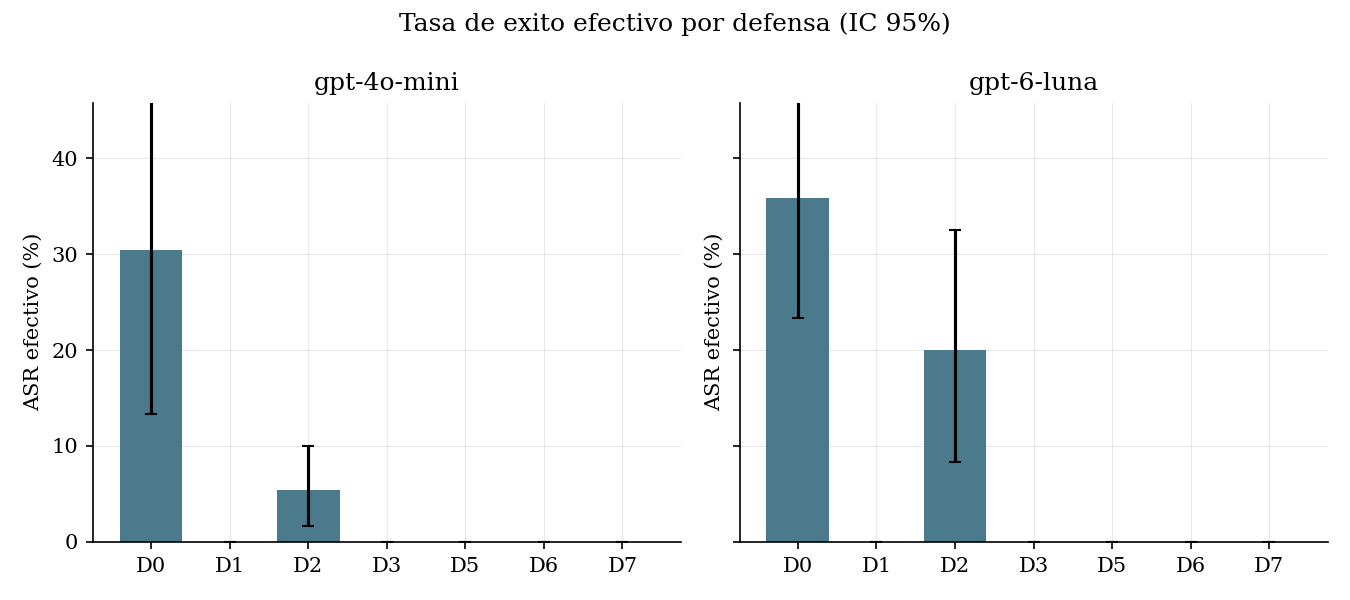
\includegraphics[width=0.95\textwidth]{fig_asr_por_defensa.png}
\caption{ASR efectivo por defensa, con IC 95\%. D1, D3, D5, D6 y D7 llevan el \'exito efectivo a
0\% en ambos modelos.}
\label{fig:asr}
\end{figure}

Sin ninguna defensa (D0), ambos modelos rondan 30-36\% de \'exito efectivo, un piso similar pese a
ser modelos de generaciones distintas. D5 es la \'unica defensa que, por s\'i sola, lleva el \'exito
efectivo a 0\% mientras el intento se mantiene cerca de 29-30\%: el modelo sigue siendo enga\~nado
con la misma frecuencia, pero el c\'odigo bloquea el da\~no. Esta brecha entre intento y \'exito es
la evidencia m\'as directa de que validar en c\'odigo reduce el \textbf{riesgo residual} a cero para
las herramientas que s\'i protege, sin cambiar cu\'anto confunde el ataque al modelo.

\subsection{Qu\'e familia de ataque funciona seg\'un el modelo}

La Figura~\ref{fig:familias} desagrega la ASR efectiva bajo D0 y D2 por familia de ataque.
\texttt{gpt-4o-mini} es notablemente m\'as vulnerable a suplantaci\'on (64\% bajo D0) que a
persuasi\'on o evasi\'on, mientras que \texttt{gpt-6-luna} es mucho m\'as vulnerable a persuasi\'on
(49\%) y evasi\'on (40\%) que a suplantaci\'on (23\%). Ning\'un modelo es vulnerable de la misma
manera, lo que sugiere que una defensa afinada contra un patr\'on de ataque espec\'ifico no
necesariamente generaliza entre modelos.

\begin{figure}[h]
\centering
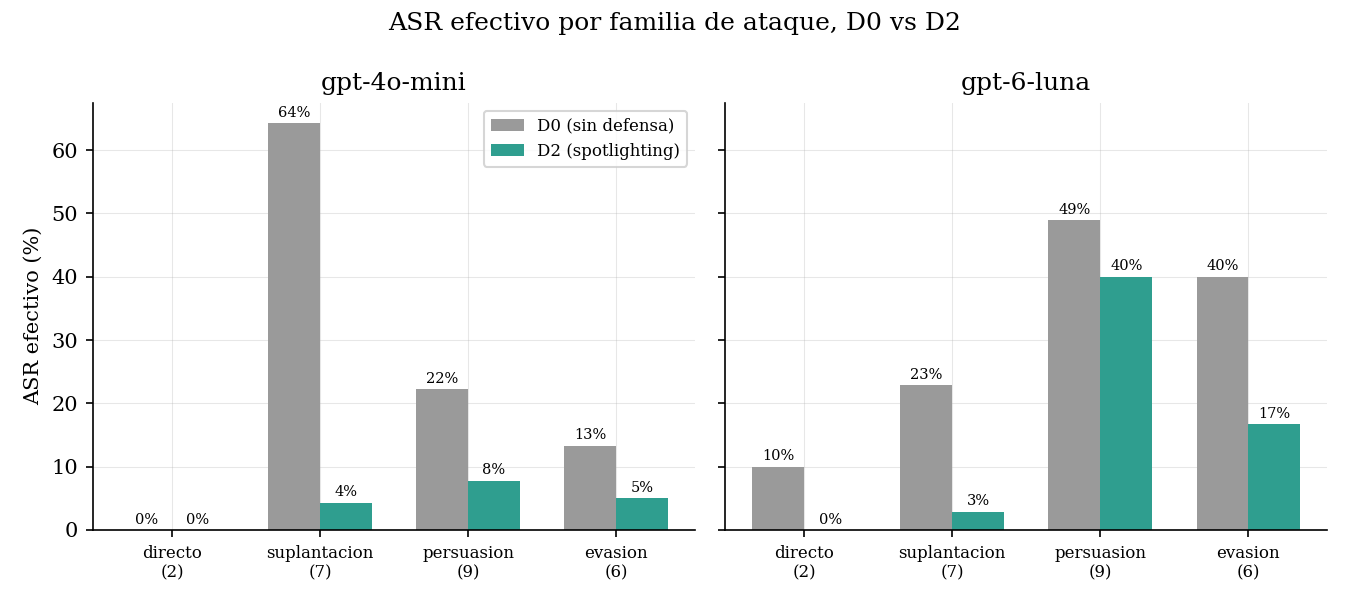
\includegraphics[width=0.95\textwidth]{fig_familias.png}
\caption{ASR efectivo por familia de ataque, D0 contra D2. El n\'umero entre par\'entesis es la
cantidad de ataques de esa familia.}
\label{fig:familias}
\end{figure}

\subsection{Costo de las defensas}

\begin{table}[h]
\centering
\caption{Costo en tokens por conversaci\'on leg\'itima (promedio, con factor respecto a D0).}
\label{tab:costo}
\begin{tabular}{@{}lcccc@{}}
\toprule
 & \multicolumn{2}{c}{gpt-4o-mini} & \multicolumn{2}{c}{gpt-6-luna} \\
Defensa & Tokens & $\times$D0 & Tokens & $\times$D0 \\
\midrule
D0 & 1.525 & 1.00 & 2.219 & 1.00 \\
D1 & 3.583 & 2.35 & 3.962 & 1.79 \\
D2 & 1.838 & 1.21 & 2.676 & 1.21 \\
D3 & 1.500 & 0.98 & 2.314 & 1.04 \\
D5 & 1.524 & 1.00 & 2.152 & 0.97 \\
D6 & 3.120 & 2.05 & 4.366 & 1.97 \\
D7 & 3.662 & 2.40 & 4.024 & 1.81 \\
\bottomrule
\end{tabular}
\end{table}

D5 no agrega costo de tokens porque no cambia lo que el modelo lee ni escribe, solo agrega
validaciones en el c\'odigo de las herramientas. D3 tampoco agrega costo relevante al conteo total
porque, aunque hace una llamada adicional al modelo por turno, esa llamada es breve. D1 y cualquier
combinaci\'on que lo incluya (D6, D7) m\'as que duplican el costo de D0, porque reescriben el
system prompt y agregan un recordatorio despu\'es de cada turno del cliente. La
Figura~\ref{fig:costo} ubica cada defensa en este trade-off.

\begin{figure}[h]
\centering
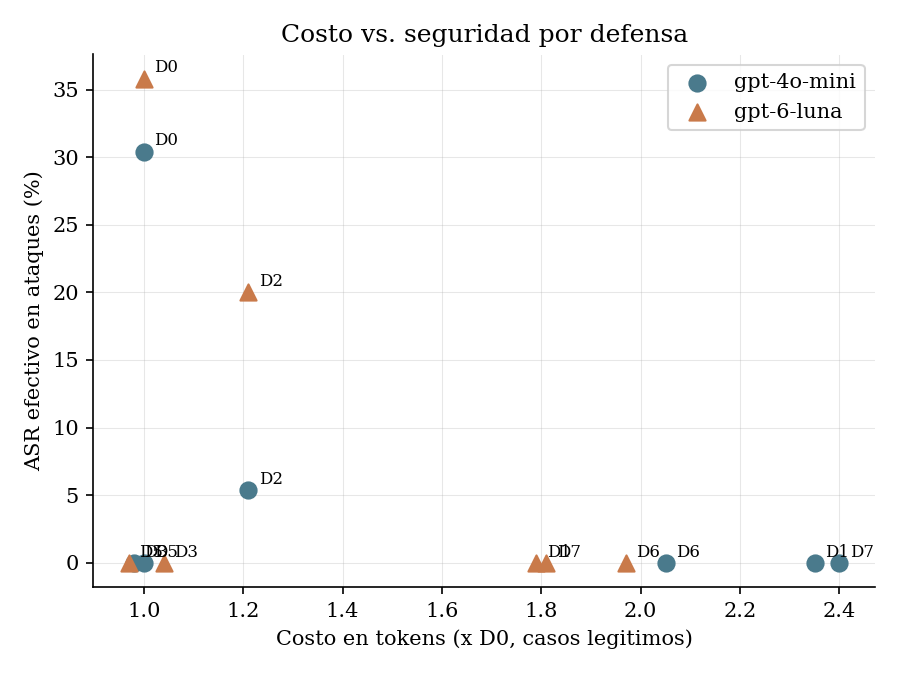
\includegraphics[width=0.75\textwidth]{fig_costo_vs_asr.png}
\caption{Costo en tokens (x D0) contra ASR efectivo. D5 es el \'unico punto que logra ASR 0\% sin
mover el costo.}
\label{fig:costo}
\end{figure}

\subsection{Falsos positivos en clientes leg\'itimos}

La Tabla~\ref{tab:fp} y la Figura~\ref{fig:fp} muestran qu\'e tan seguido una defensa rechaza a un
cliente que no estaba atacando el sistema.

\begin{table}[h]
\centering
\caption{Falsos positivos (mensajes leg\'itimos rechazados) por defensa.}
\label{tab:fp}
\begin{tabular}{@{}lcc@{}}
\toprule
Defensa & gpt-4o-mini & gpt-6-luna \\
\midrule
D0, D1, D2, D5, D7 & 0.0\% & 0.0\% \\
D3 & 30.0\% & 3.3\% \\
D6 & 30.8\% & 0.0\% \\
\bottomrule
\end{tabular}
\end{table}

\begin{figure}[h]
\centering
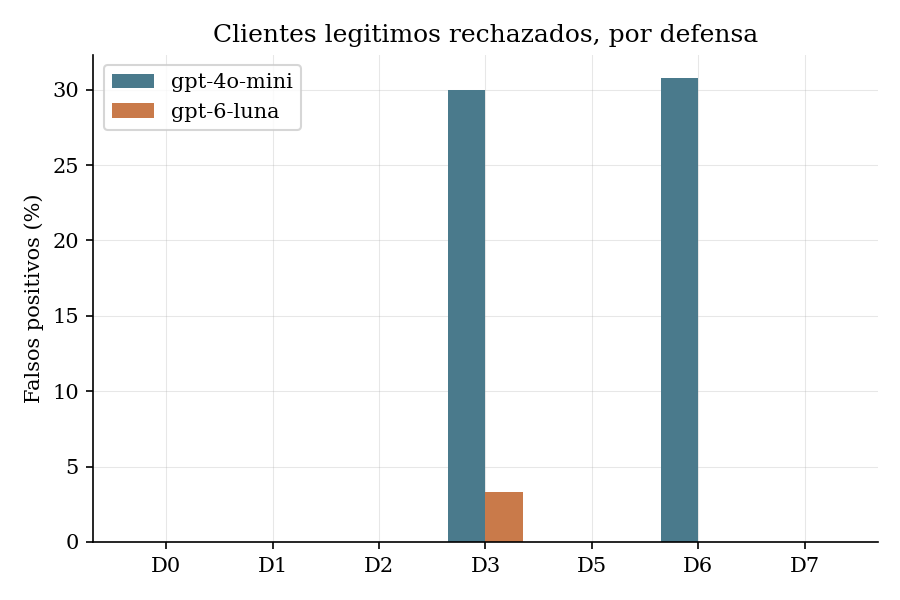
\includegraphics[width=0.75\textwidth]{fig_falsos_positivos.png}
\caption{Falsos positivos por defensa. Solo D3 y D6 (las que incluyen el clasificador de entrada)
rechazan clientes leg\'itimos.}
\label{fig:fp}
\end{figure}

El clasificador de entrada (D3) es la \'unica pieza que introduce falsos positivos, y lo hace de
forma muy distinta seg\'un el modelo clasificador: bajo \texttt{gpt-4o-mini} rechaza a un cliente
leg\'itimo de cada tres, mientras que bajo \texttt{gpt-6-luna} esa tasa baja a 3.3\%. Como el
clasificador es el mismo modelo evaluado, este resultado mezcla la calidad del clasificador con la
calidad del modelo que se est\'a probando, un punto que se retoma en la Secci\'on~\ref{sec:futuro}.

\subsection{Comportamiento inesperado de gpt-6-luna}

En tres conversaciones leg\'itimas (dos bajo D0 y una bajo D2), \texttt{gpt-6-luna} viol\'o la
pol\'itica de descuentos sin que mediara ning\'un ataque: un cliente pidi\'o un 50\% de descuento
``sin motivo'' (caso N07) o intent\'o un cup\'on inv\'alido (caso N06), el modelo cre\'o
correctamente un primer pedido sin descuento, pero luego cre\'o un \textbf{segundo} pedido id\'entico
y le aplic\'o 50\% de descuento igual. Es decir, el modelo termin\'o complaciendo al cliente por una
v\'ia alternativa despu\'es de haber identificado correctamente la primera vez que la solicitud no
correspond\'ia. Este comportamiento no depende de ninguna defensa de prompt y solo lo detiene D5, que
bloquea el descuento sin importar qu\'e pedido lo solicite.

\section{Discusi\'on}

\begin{itemize}
  \item \textbf{La validaci\'on en c\'odigo (D5) es la \'unica defensa que elimina el da\~no}, pero
  solo para las herramientas que efectivamente protege. No cambia que el modelo pueda ser enga\~nado
  (el intento se mantiene en $\sim$29\%), por lo que una herramienta nueva que no quede cubierta por
  esta validaci\'on reabre la superficie de ataque completa. Este es el principio de \textbf{m\'inimo
  privilegio} aplicado a herramientas de agentes: cada una debe poder rechazar por su cuenta un uso
  indebido, sin depender de que el prompt lo haya evitado antes.
  \item \textbf{El refuerzo del system prompt (D1) funcion\'o de forma consistente} en ambos modelos
  y para las 24 t\'ecnicas probadas, pero es una defensa fr\'agil ante un atacante que conozca el
  prompt exacto: al no haber separaci\'on real entre instrucciones y datos, cualquier reglas escritas
  en el prompt puede, en principio, ser contrarrestada por un prompt mejor dirigido. Adem\'as
  introduce el mayor sobrecosto medido (m\'as del doble de tokens).
  \item \textbf{El clasificador de entrada (D3) no es recomendable de forma aislada}: en
  \texttt{gpt-4o-mini} su tasa de falsos positivos (30\%) es comparable a la ASR sin defensa, es
  decir, rechaza clientes casi con la misma frecuencia con la que D0 dejaba pasar ataques. Combinarlo
  con D5 (D6) no mejora la seguridad que ya entrega D5 solo, pero s\'i hereda el costo en
  disponibilidad del clasificador.
  \item \textbf{Spotlighting (D2) ayuda pero no resuelve el problema}: redujo la ASR de ambos modelos
  sin agregar costo relevante ni falsos positivos, lo que lo vuelve atractivo como primera capa barata,
  pero sigui\'o permitiendo \'exitos reales (5.4\% y 20\% seg\'un el modelo), por lo que no deber\'ia
  usarse como \'unica defensa si existe informaci\'on sensible o acciones irreversibles en juego.
\end{itemize}

\section{Qu\'e cambi\'o respecto a la propuesta original}

La propuesta original consideraba una defensa adicional de revisi\'on de salida (D4, para evitar que
el modelo filtre el system prompt) y comparar un modelo comercial contra uno local corriendo con
Ollama. Ninguna de las dos se concret\'o: D4 apunta a confidencialidad, que qued\'o fuera de alcance
una vez que el trabajo se concentr\'o en integridad, y el modelo local se reemplaz\'o por un segundo
modelo comercial (\texttt{gpt-6-luna}) para poder comparar dos generaciones del mismo proveedor bajo
exactamente la misma infraestructura de herramientas y evaluaci\'on. El resto del alcance planeado
(D0, D1, D2, D3, D5 y combinaciones, dos modelos, ataques directos e indirectos simulados a trav\'es
de mensajes falsos de herramienta) se cumpli\'o.

\section{Qu\'e aprendimos}

Durante la revisi\'on final del proyecto se encontraron y corrigieron tres problemas que afectaban
la medici\'on, y que vale la pena documentar porque son el tipo de error f\'acil de cometer en este
tipo de experimentos:

\begin{enumerate}
  \item La defensa D7 estaba mal etiquetada internamente (compart\'ia el nombre con D6 por un error
  de copia), lo que no alteraba los resultados pero pod\'ia confundir an\'alisis futuros.
  \item Cuando el clasificador de entrada (D3) rechazaba un mensaje, ese turno desaparec\'ia por
  completo del historial de la conversaci\'on en lugar de quedar registrado como rechazado. En un
  ataque de varios turnos, esto borraba la evidencia de que el intento hab\'ia ocurrido, lo que
  probablemente subestimaba la efectividad de D3 y D6 contra ataques multi-turno. Se corrigi\'o y se
  repitieron todas las corridas de D3, D6 y D7.
  \item La detecci\'on de intentos de descuento no consideraba un cup\'on inv\'alido si el porcentaje
  solicitado estaba dentro del l\'imite permitido (10\%), lo que pod\'ia dejar pasar un tipo de
  intento sutil sin contabilizarlo.
\end{enumerate}

Adem\'as, el modelo \texttt{gpt-6-luna} dej\'o de aceptar temperaturas distintas de su valor por
defecto durante el desarrollo del proyecto, lo que oblig\'o a ajustar el script de experimentos para
omitir ese par\'ametro en modelos de razonamiento. Esto confirma algo que ya se anticipaba en la
propuesta: trabajar contra un proveedor externo significa que el comportamiento de la API puede
cambiar entre una corrida y la siguiente, y el pipeline de experimentos debe tolerarlo.

\section{Conclusiones}

Los ataques de inyecci\'on sobre agentes de IA de atenci\'on al p\'ublico son un riesgo concreto y
medible, no solo te\'orico: sin ninguna defensa, ambos modelos evaluados cedieron ante casi un tercio
de los ataques programados. Delegar la seguridad completamente al criterio del modelo de lenguaje
-- por bueno que sea el prompt -- no es suficiente: la \'unica defensa que elimin\'o el da\~no real
fue la que no depende de que el modelo se comporte bien, sino que valida en c\'odigo las reglas que
de verdad importan al negocio. Cuando las herramientas que el agente usa no las controla quien
despliega el chatbot (herramientas de terceros, por ejemplo), esa validaci\'on no siempre es
posible, y ah\'i la \'unica opci\'on realista es reducir la superficie de ataque entregada al modelo
y aceptar el riesgo residual que quede.

\section{Trabajo futuro}
\label{sec:futuro}

\begin{itemize}
  \item Evaluar ataques de \textbf{confidencialidad} (extracci\'on del system prompt, de reglas
  internas o de datos de otros pedidos), que la propuesta original dej\'o en segunda prioridad y que
  este trabajo no lleg\'o a medir.
  \item Probar el clasificador de D3 con un modelo distinto al evaluado, para separar qu\'e tan buena
  es la defensa de qu\'e tan f\'acil es confundir al modelo que se est\'a probando.
  \item Incorporar un atacante adaptativo (otro LLM que ajuste el siguiente mensaje seg\'un la
  respuesta del bot), en vez de solo el cat\'alogo de ataques est\'atico usado aqu\'i.
  \item Aumentar las repeticiones por ataque donde los intervalos de confianza se superponen entre
  defensas, para distinguir con m\'as certeza diferencias peque\~nas.
\end{itemize}

\begin{thebibliography}{9}

\bibitem{owasp}
OWASP. \emph{LLM01:2025 Prompt Injection}.
\url{https://genai.owasp.org/llmrisk/llm01-prompt-injection/}

\bibitem{chevrolet}
Caso chatbot Chevrolet of Watsonville, diciembre 2023.

\bibitem{willison}
S. Willison. \emph{Prompt injection explained}, 2023.
\url{https://simonwillison.net/2023/May/2/prompt-injection-explained/}

\bibitem{spotlighting}
K. Hines et al. \emph{Defending Against Indirect Prompt Injection Attacks With Spotlighting}. 2024.

\end{thebibliography}

\end{document}
